\documentclass{beamer}[10]

\usepackage{graphicx}
\usepackage{xcolor}
\usepackage{tabto}
%\usepackage{beamerthemesplit}
\usepackage{tikz}
\usepackage{cancel}
\usepackage{verbatim}
\usepackage{fancybox}
\usepackage{enumerate}
\usepackage{amsmath,amssymb,amsthm,textcomp,mathtools}
\usepackage[super]{nth}
\usepackage[amssymb]{SIunits}
\usepackage{booktabs}
\usepackage{cancel}
\usepackage{bm}
\usepackage[utf8]{inputenc}
\usepackage{tabularx}
\usepackage{ragged2e}
\newcolumntype{Y}{ >{\RaggedRight\arraybackslash}X}
\usetikzlibrary{arrows,shapes}
\newcommand\T{\rule{0pt}{2.6ex}}
\newcommand\B{\rule[-1.2ex]{0pt}{0pt}}
\definecolor{UUcrimson}{RGB}{204,0,0}
\mode<presentation>
{ \usetheme{default}
  \usecolortheme[named=UUcrimson]{structure}
  \useinnertheme{circles}
  \setbeamercovered{transparent}
  \setbeamertemplate{blocks}[rounded]
  \usefonttheme[onlymath]{serif}
  \setbeamertemplate{navigation symbols}{}
  \setbeamertemplate{footline}[page number]
  \setbeamertemplate{navigation symbols}{}
  \setbeamercolor{section in toc}{fg=black,bg=white}
  \setbeamercolor{alerted text}{fg=UUcrimson!80!gray}
  \setbeamercolor*{palette primary}{fg=white,bg=UUcrimson}
  \setbeamercolor*{palette secondary}{fg=UUcrimson!70!black,bg=gray!15!white}
  \setbeamercolor*{palette tertiary}{bg=UUcrimson!80!black,fg=gray!10!white}
  \setbeamercolor*{palette quaternary}{fg=UUcrimson,bg=gray!5!white}
  \setbeamercolor*{palette sidebar primary}{fg=UUcrimson!10!black}
  \setbeamercolor*{palette sidebar secondary}{fg=white}
  \setbeamercolor*{palette sidebar tertiary}{fg=UUcrimson!50!black}
  \setbeamercolor*{palette sidebar quaternary}{fg=gray!10!white}
  \setbeamercolor{titlelike}{parent=palette primary,fg=white}
  \setbeamercolor{frametitle}{bg=UUcrimson}
  \setbeamercolor{frametitle right}{bg=UUcrimson}
  \setbeamercolor*{separation line}{}
  \setbeamercolor*{fine separation line}{}
}

\usetikzlibrary{backgrounds}
\makeatletter
\tikzstyle{every picture}+=[remember picture]
\tikzset{%
  fancy quotes/.style={
    text width=\fq@width pt,
    align=justify,
    inner sep=1em,
    anchor=north west,
    minimum width=\linewidth,
    font=\itshape
  },
  fancy quotes width/.initial={.8\linewidth},
  fancy quotes marks/.style={
    scale=8,
    text=white,
    inner sep=0pt,
  },
  fancy quotes opening/.style={
    fancy quotes marks,
  },
  fancy quotes closing/.style={
    fancy quotes marks,
  },
  fancy quotes background/.style={
    show background rectangle,
    inner frame xsep=0pt,
    background rectangle/.style={
      fill=gray!25,
      rounded corners,
    },
  }
}
\newenvironment{fancyquotes}[1][]{%
\noindent
\tikzpicture[fancy quotes background]
\node[fancy quotes opening,anchor=north west] (fq@ul) at (0,0) {``};
\tikz@scan@one@point\pgfutil@firstofone(fq@ul.east)
\pgfmathsetmacro{\fq@width}{\linewidth - 2*\pgf@x}
\node[fancy quotes,#1] (fq@txt) at (fq@ul.north west) \bgroup}
{\egroup;
\node[overlay,fancy quotes closing,anchor=east] at (fq@txt.south east) {''};
\endtikzpicture}
\makeatother


\usetikzlibrary{backgrounds}
\makeatletter
\tikzstyle{every picture}+=[remember picture]
\tikzset{%
  fancy defs/.style={
    text width=\fq@width pt,
    align=justify,
    inner sep=0.25em,
    anchor=north west,
    minimum width=\linewidth,
    font=\itshape
  },
  fancy defs width/.initial={.8\linewidth},
  fancy defs marks/.style={
    scale=8,
    text=white,
    inner sep=0pt,
  },
  fancy defs opening/.style={
    fancy defs marks,
  },
  fancy defs closing/.style={
    fancy defs marks,
  },
  fancy defs background/.style={
    show background rectangle,
    inner frame xsep=0pt,
    background rectangle/.style={
      fill=gray!25,
      rounded corners,
    },
  }
}
\newenvironment{fancydefs}[1][]{%
\noindent
\tikzpicture[fancy defs background]
\node[fancy defs opening,anchor=north west] (fq@ul) at (0,0) {};
\tikz@scan@one@point\pgfutil@firstofone(fq@ul.east)
\pgfmathsetmacro{\fq@width}{\linewidth - 2*\pgf@x}
\node[fancy defs,#1] (fq@txt) at (fq@ul.north west) \bgroup}
{\egroup;
\node[overlay,fancy defs closing,anchor=east] at (fq@txt.south east) {};
\endtikzpicture}
\makeatother
\usepackage{scalerel}[2014/03/10]
\usepackage{stackengine}
\usepackage{empheq}
\newcommand*\widefbox[1]{\fbox{\hspace{0.5em}#1\hspace{0.5em}}}

\newcommand\reallywidetilde[1]{\ThisStyle{%
  \setbox0=\hbox{$\SavedStyle#1$}%
  \stackengine{-.1\LMpt}{$\SavedStyle#1$}{%
    \stretchto{\scaleto{\SavedStyle\mkern.2mu\sim}{.5467\wd0}}{.4\ht0}%
%    .2mu is the kern imbalance when clipping white space
%    .5467++++ is \ht/[kerned \wd] aspect ratio for \sim glyph
  }{O}{c}{F}{T}{S}%
}}
\usepackage{media9}

\logo{
\includegraphics[width=0.75cm]{logo.jpg}}
\author[Gibbs]{Dr. Jeremy A. Gibbs}
\institute{Department of Mechanical Engineering\\University of Utah}
\date{Spring 2017}
\title{Environmental Fluid Dynamics: Lecture 20}
% colors
\usepackage[loadonly]{enumitem}
\newcommand{\ihat}{\boldsymbol{\hat{\imath}}}
\newcommand{\jhat}{\boldsymbol{\hat{\jmath}}}
\newcommand{\khat}{\boldsymbol{\hat{k}}}
\definecolor{colororange}{HTML}{E65100} % orange
\definecolor{colordgray}{HTML}{795548} % dark gray for note
\definecolor{colorhgray}{HTML}{212121} % heavy dark gray for normal text
\definecolor{colorgreen}{HTML}{009688} % green
\definecolor{colorwhite}{HTML}{FFFFFF} % background white
\definecolor{colorlgray}{HTML}{F5F3EE} % background light gray
\definecolor{colorblue}{HTML}{0277BB} % blue
\definecolor{colorred}{HTML}{CC0000} % red
\newcommand{\fontsizeone}{1.9em}
\usepackage{esvect}
\setbeamertemplate{caption}{\raggedright\insertcaption\par}
\newcommand{\framecard}[2][colorgreen]{
  {\setbeamercolor{background canvas}{bg=#1}
    \begin{frame}[plain]
    \vfill
    \begin{center}
     {#2}
    \end{center}
    \vfill
    \end{frame}
  }
}
\begin{document}

%----------------------------------------------------------------------------------------
%	TITLE & TOC SLIDES
%----------------------------------------------------------------------------------------

\begin{frame} 
  \titlepage
\end{frame}

%------------------------------------------------

\begin{frame}
\frametitle{Overview}
\tableofcontents
\end{frame}

%------------------------------------------------
\section{Similarity Theory} %
%------------------------------------------------
\framecard[colorred]{{\color{white}\Huge Similarity Theory}}
%------------------------------------------------
\subsection{Overview}
%------------------------------------------------
\begin{frame}{Similarity Theory}
\begin{itemize}
	\item \textbf{Goal:} We want to describe physical processes in the ABL.
	\item \textbf{Problem:} We lack understanding of the underlying physics.
	\item \textbf{Solution:} Derive empirical relationships b/t ABL variables.
	\item \textbf{Tool:} Similarity theory - group variables, create relationships.
\end{itemize}
\end{frame}
%------------------------------------------------
\begin{frame}{Similarity Theory}
\begin{itemize}
	\item Similarity theory is based on placing variables into dimensionless groups.
	\item We will use Buckingham Pi theory to do this.
	\item The goal is to properly group the variables such that we can create universal relationships between them.
\end{itemize}
\end{frame}
%------------------------------------------------
\begin{frame}{Similarity Theory}
\textbf{Four Steps to Develop Similarity Theory}
\begin{itemize}
	\item Choose relevant variables
	\item Organize variables into dimensionless groups
	\item Use experimental data to determine values of dimensionless groups
	\item Create bets-fit curve to describe the relationship between the variables
\end{itemize}
\end{frame}
%------------------------------------------------
\begin{frame}{Similarity Theory}
\begin{itemize}
	\item Result is an empirical equation or curves that show the same shape (i.e., they look self-similar - thus, similarity theory).
	\item We hope the result is universal so that we can apply it to other situations different to our experiment.
	\item The derived equations are called similarity relationships.
	\item These relationships are usually applied to steady-state situations.
	\item Think of similarity theory as a zero-order closure - we can use them to diagnose values of mean wind, temperature, and moisture as a function of height without making any assumptions regarding turbulence closure
\end{itemize}
\end{frame}
%------------------------------------------------
\subsection{Buckingham Pi Theory}
%------------------------------------------------
\begin{frame}{Buckingham Pi Theory}
\begin{itemize}
	\item Buckingham (1914) proposed a systematic approach for dimensional analysis.
	\item Buckingham Pi Theory represents an optimal approach to determine a dependent variable in a physical problem.
	\item If we can identify $m-1$ parameters that govern a dependent variable, and if $n$ is the number of dimensions, then:
	\begin{itemize}
		\item $m-n$ independent dimensionless quantities ($\pi$ groups) are formed (cannot be made from other $\pi$ groups)
		\item $m-n$ independent dimensionless quantities are functionally related so that the dependent variable can be taken as a function of the governing parameters.
	\end{itemize}
	\item The requires a grasp of a problem's physics.
	\end{itemize}
\end{frame}
%------------------------------------------------
\begin{frame}{Buckingham Pi Theory}
\textbf{Buckingham Pi Theory - A procedure to group variables into dimensionless groups}
\begin{enumerate}
	\item Select variables relevant to the problem
	\item Find the dimensions of each variables and express in terms of fundamental dimensions: (e.g., length, mass, time, temp.)
	\item Count the number of fundamental dimensions
	\item Pick subset of the original variables as ``key'' variables, subject to these restrictions:
	\begin{itemize}
		\item The number of key variables must be equal to the number of fundamental dimensions.
		\item All fundamental dimensions must be represented in the key variables
		\item No dimensionless group may be possible from any combination of the key variables
	\end{itemize}
\end{enumerate}
\end{frame}
%------------------------------------------------
\begin{frame}{Buckingham Pi Theory}
\textbf{Buckingham Pi Theory - A procedure to group variables into dimensionless groups}
\begin{enumerate}
	\setcounter{enumi}{4}
	\item Form dimensionless equations of the remaining variables in terms of the key variables
	\item Solve for powers of the terms in the equations to yield dimensionally consistent equations
	\item Divide the left hand side of each equation by the right to get dimensionless ($\pi$) group. The number of $\pi$ groups will always equal the number of variables minus the number of dimensions.
\end{enumerate}
\end{frame}
%------------------------------------------------
\begin{frame}{Buckingham Pi Theory: Example}
\textbf{Consider flow through a pipe. How does $\tau$ vary?}
\begin{enumerate}
	\item We hypothesize that the important variables are fluid density, dynamic viscosity, velocity, shear stress, pipe diameter, and pipe roughness
	\item The fundamental dimensions of these variables are:
	\begin{align*}
	&\text{fluid density}     & \rho & &\mathrm{M\ L^{-3}}\\
	&\text{dynamic viscosity} & \mu  & &\mathrm{M\ L^{-1}\ T^{-1}}\\
	&\text{velocity}          & U    & &\mathrm{L\ T^{-1}}\\
	&\text{shear stress}      & \tau & &\mathrm{M\ L^{-1}\ T^{-2}}\\
	&\text{pipe diameter}     & D    & &\mathrm{L}\\
	&\text{pipe roughness}    & z_0  & &\mathrm{L}
	\end{align*}
\end{enumerate}
\end{frame}
%------------------------------------------------
\begin{frame}{Buckingham Pi Theory: Example}
\textbf{Consider flow through a pipe. How does $\tau$ vary?}
\begin{enumerate}
\setcounter{enumi}{2}
	\item There are 3 fundamental dimensions: $\mathrm{M, L, T}$
	\item We need 3 key variables. Let's choose $\rho$, $D$, and $U$.
	\item Now we form dimensionless equations for $\mu$, $\tau$, and $z_0$ in terms of $\rho$, $D$, and $U$
	\begin{align*}
		\tau &= \rho^a D^b U^c\\
		\mu  &= \rho^d D^e U^f\\
		z_0  &= \rho^g D^h U^i\\
	\end{align*}
\end{enumerate}
\end{frame}
%------------------------------------------------
\begin{frame}{Buckingham Pi Theory: Example}
\textbf{Consider flow through a pipe. How does $\tau$ vary?}
\begin{enumerate}
\setcounter{enumi}{5}
	\item Now we solve for the exponents. Let's look at $\tau$:
	\begin{align*}
	\tau &= \rho^a D^b U^c\\
	\mathrm{M\ L^{-1}\ T^{-2}} &= (\mathrm{M\ L^{-3}})^a (L)^b (\mathrm{L\ T^{-1}})^c\\
	\mathrm{M\ L^{-1}\ T^{-2}} &= \mathrm{M}^a\ \mathrm{L}^{-3a + b + c}\ \mathrm{T}^{-c}
	\end{align*}
	We must match dimensions
	$$\mathrm{M}: 1 = a \qquad \mathrm{L}: -1 = -3a+b+c \qquad \mathrm{T}: -2 = -c$$
	We solve for the unknowns to yield:
	$$a=1 \qquad b=0 \qquad c=2$$
\end{enumerate}
\end{frame}
%------------------------------------------------
\begin{frame}{Buckingham Pi Theory: Example}
\textbf{Consider flow through a pipe. How does $\tau$ vary?}
\begin{enumerate}
\setcounter{enumi}{5}
	\item Thus, our dimensionally consistent equation is:
	$$\tau = \rho^1 D^0 U^2 = \rho U^2$$
	Similarly, we find that:
	$$\mu = \rho U D \qquad z_0 = D$$
	\item Now we divide the left by the right side to get our $\pi$ groups
	$$\pi_1 = \frac{\tau}{\rho U^2} \qquad \pi_2 = \frac{\mu}{\rho U D} \qquad \pi_3 = \frac{z_0}{D}$$
	Note that $\pi_1$ is the drag coefficient $C_D$, $\pi_2$ is inverse Reynolds number $\mathrm{Re}$, and $\pi_3$ is relative roughness.
\end{enumerate}
\end{frame}
%------------------------------------------------
\subsection{Scaling Variables}
%------------------------------------------------
\begin{frame}{Scaling Variables}
\begin{itemize}
	\item For similarity theory, we want variables that represent forcings on the boundary layer (e.g., fluxes).
	\item Some key variables appear often and are called scaling variables.
	\item Generally, we want one length scale, one velocity scale, and if needed a temperature/moisture scale (usually no time scale since it can be made from length and velocity scales).
	\item Some variables always appear grouped, which allows for the creation of new scaling variables based on their combination.
	\end{itemize}
\end{frame}
%------------------------------------------------
\begin{frame}{Scaling Variables}
\begin{itemize}
	\item Some common scaling variables for the atmosphere:
	\begin{align*}
	u_* &= (-\overline{w^\prime u^\prime})^{1/2} \\
	\theta_* &= \frac{-(\overline{w^\prime \theta^\prime})}{u_*}\\
	\theta_{v*} &= \frac{-(\overline{w^\prime \theta_v^\prime})}{u_*}\\
	q_* &= \frac{-(\overline{w^\prime q^\prime})}{u_*}\\
	b_* &= \frac{-(\overline{w^\prime b^\prime})}{u_*}
	\end{align*}
	\end{itemize}
\end{frame}
%------------------------------------------------
\begin{frame}{Scaling Variables}
\begin{itemize}
	\item Let's consider the signs of these scaling variables depending on static stability:
	\begin{align*}
	\text{unstable} &\rightarrow \overline{w^\prime b^\prime} > 0, \partial b/\partial z < 0, b_* < 0\\
	\text{neutral} &\rightarrow \overline{w^\prime b^\prime} = 0, \partial b/\partial z = 0, b_* = 0\\
	\text{stable} &\rightarrow \overline{w^\prime b^\prime} < 0, \partial b/\partial z > 0, b_* > 0\\
	\end{align*}
	\item Notice how the scaling terms are aligned with the gradients.
	\end{itemize}
\end{frame}
%------------------------------------------------
\subsection{Monin-Obukhov Similarity Theory}
%------------------------------------------------
\begin{frame}{Monin-Obukhov Similarity Theory}
\begin{itemize}
	\item Theory developed for the atmosphere by Monin-Obukhov (1954) based on dimensional analysis.
	\item Monin-Obukhov Similarity Theory (MOST) suggests that there are four parameters governing quasi-steady-state turbulence immediately above a flat, horizontally- homogeneous surface
	\begin{align*}
		\ell = \kappa z &\qquad \text{length scale of turbulence}\\
		u_* & \qquad \text{friction velocity}\\
		B_0=\overline{w^\prime b^\prime} & \qquad \text{buoyancy flux}\\
		\partial \overline{u}/\partial z & \qquad \text{velocity gradient}
	\end{align*}
	\item Note: $\kappa$ is the von K\'{a}rm\'{a}n ``constant'', which is a dimensionless constant of proportionality introduced to relate the turbulence length scale and height above the surface. A typical value is $\kappa = 0.4$.
	\end{itemize}
\end{frame}
%------------------------------------------------
\begin{frame}{Monin-Obukhov Similarity Theory}
\textbf{It is also important to consider what we ignored:}
	\begin{itemize}
		\item \textit{boundary layer depth}: assume largest eddies do not greatly influence eddies near the surface
		\item \textit{mean wind}: turbulence must be invariant to Galilean transformations, and the mean wind is not 
		\item \textit{rotational effects}: turbulence Coriolis force is very small
		\item \textit{molecular effects}: turbulence Reynolds number is very large
		\item \textit{roughness elements $z_0$}: assume $z \gg z_0$
	\end{itemize}
\end{frame}
%------------------------------------------------
\begin{frame}{Monin-Obukhov Similarity Theory}
	\begin{itemize}
		\item The fundamental dimensions of our governing variables are:
	\begin{align*}
	&\text{turbulence length scale} & \ell & &\mathrm{L}\\
	&\text{friction velocity} & u_*  & &\mathrm{L\ T^{-1}}\\
	&\text{buoyancy flux}     & B_0  & &\mathrm{L^2\ T^{-3}}\\
	&\text{velocity gradient} & \partial \overline{u}/\partial z  & &\mathrm{T^{-1}}
	\end{align*}
	\item So we have $m=4$ paramters and $n=2$ dimensions.
	\item Accordingly, we expect to have $m-n=2$ $\pi$ groups.
	\item We take group as a non-dimensionalized dependent variable and the other as the independent variable.
	\end{itemize}
\end{frame}
%------------------------------------------------
\begin{frame}{Monin-Obukhov Similarity Theory}
	\begin{itemize}
		\item Let's fidn the non-dimensionalized dependent variable
		\item There are 2 fundamental dimensions: $\mathrm{L, T}$
		\item We need 2 key variables. Let's choose $u_*$ and $\kappa z$.
	\item Form a dimensionless equation for $\partial \overline{u} /\partial z$ in terms of $u_*$ and $\kappa z$: 
	$$ \partial \overline{u} /\partial z= u_*^a\ (\kappa z)^b$$
	\item Now we solve for the exponents.
	\begin{align*}
	\partial \overline{u} /\partial z &= u_*^a\ (\kappa z)^b\\
	\mathrm{T^-1} &= (\mathrm{L\ T^{-1}})^a\ (\mathrm{L})^b\\
	\mathrm{T^-1} &= L^{a+b}\ T^{-a}
	\end{align*}
	We must match dimensions
	$$\mathrm{L}: 0 = a+b \qquad \mathrm{T}: -1 = -a$$
	We solve for the unknowns to yield:
	$$a=1 \qquad b=-1$$
	\end{itemize}
\end{frame}
%------------------------------------------------
\begin{frame}{Monin-Obukhov Similarity Theory}
	\begin{itemize}
		\item Thus, our dimensionally consistent equation is:
	$$ \partial \overline{u} /\partial z = u_*^1\ (\kappa z)^{-1}$$
	\item Now we divide the left by the right side to get our $\pi$ groups
	$$\pi_1 = \frac{\kappa z}{u_*} \frac{\partial \overline{u}}{\partial z}$$
	\item This represents the non-dimensional dependent variable (vertical gradient of velocity)
	\end{itemize}
\end{frame}
%------------------------------------------------
\begin{frame}{Monin-Obukhov Similarity Theory}
	\begin{itemize}
		\item Now, let's find the independent variable.
		\item There are 2 fundamental dimensions: $\mathrm{L, T}$
		\item We need 2 key variables. Let's choose $u_*$ and $B_0$.
	\item Form a dimensionless equation for $\ell$ in terms of $u_*$ and $B_0$: $$
		\ell = \kappa z = u_*^a B_0^b$$
	\item Now we solve for the exponents.
	\begin{align*}
	\kappa z &= u_*^a B_0^b\\
	\mathrm{L} &= (\mathrm{L\ T^{-1}})^a\ (\mathrm{L^2\ T^{-3}})^b\\
	\mathrm{L} &= L^{a+2b}\ T^{-a-3b}
	\end{align*}
	We must match dimensions
	$$\mathrm{L}: 1 = a+2b \qquad \mathrm{T}: 0 = -a-3b$$
	We solve for the unknowns to yield:
	$$a=3 \qquad b=-1$$
	\end{itemize}
\end{frame}
%------------------------------------------------
\begin{frame}{Monin-Obukhov Similarity Theory}
	\begin{itemize}
		\item Thus, our dimensionally consistent equation is:
	$$\kappa z = u_*^3\ B_0^{-1}$$
	\item Now we divide the left by the right side to get our $\pi$ groups
	$$\pi_2 = \frac{\kappa z B_0}{u_*^3}$$
	\item Remember that we said some scaling variables always appear in a particular grouping? Here we define a new scaling variable called the Obukhov length,
	$$L=-\frac{u_*^3}{\kappa B_0}$$
	\item Thus, 
	$$\pi_2 = -\frac{z}{L}$$
	\end{itemize}
\end{frame}
%------------------------------------------------
\begin{frame}{Monin-Obukhov Similarity Theory}
\textbf{Aside: Obukhov Length}
	\begin{itemize}
		\item $|L|$ is interpreted as the height at which buoyancy effects become dynamically important.
		\item Neutral conditions: $L\rightarrow \infty \Rightarrow z/L = 0$
		\item Stable conditions: $L>0$
		\item Unstable conditions: $L<0$
		\item In the absence of surface stress (no mean flow), $L=0$
	\end{itemize}
\end{frame}
%------------------------------------------------
\begin{frame}{Monin-Obukhov Similarity Theory}
	\begin{itemize}
		\item The two $\pi$ groups are functionally related, thus
		$$\frac{\kappa z}{u_*} \frac{\partial \overline{u}}{\partial z} = \phi_m \left(\frac{z}{L} \right)$$
		where $\phi_m$ is a universal function of $\zeta = z/L$
		\item Similarly, we can show that
		\begin{align*}
			\frac{\kappa z}{\theta_*} \frac{\partial \overline{\theta}}{\partial z} &= \phi_h \left(\zeta \right)
			& \quad & \frac{\kappa z}{\theta_{v*}} \frac{\partial \overline{\theta_v}}{\partial z} = \phi_v \left(\zeta \right)\\ \frac{\kappa z}{b_*} \frac{\partial \overline{b}}{\partial z} &= \phi_b \left(\zeta \right) 
			& \quad & \frac{\kappa z}{q_{*}} \frac{\partial \overline{q}}{\partial z} = \phi_q \left(\zeta \right)
		\end{align*}
	Often we assume that $\phi_h = \phi_v = \phi_b = \phi_q$ 
	\item Thus, when normalized by $z,L,u_*, \theta_*, \theta_{v*}, b_*, q_*$, gradients of mean turbulent quantities are functions of only $\zeta=z/L$!
	\end{itemize}
\end{frame}
%------------------------------------------------
\begin{frame}{Monin-Obukhov Similarity Theory}
	\begin{itemize}
		\item We need formulations for our universal similarity functions
		\item Many empirical forms have been formulated using data from the famous 1968 Kansas experiment.
		\begin{figure}
		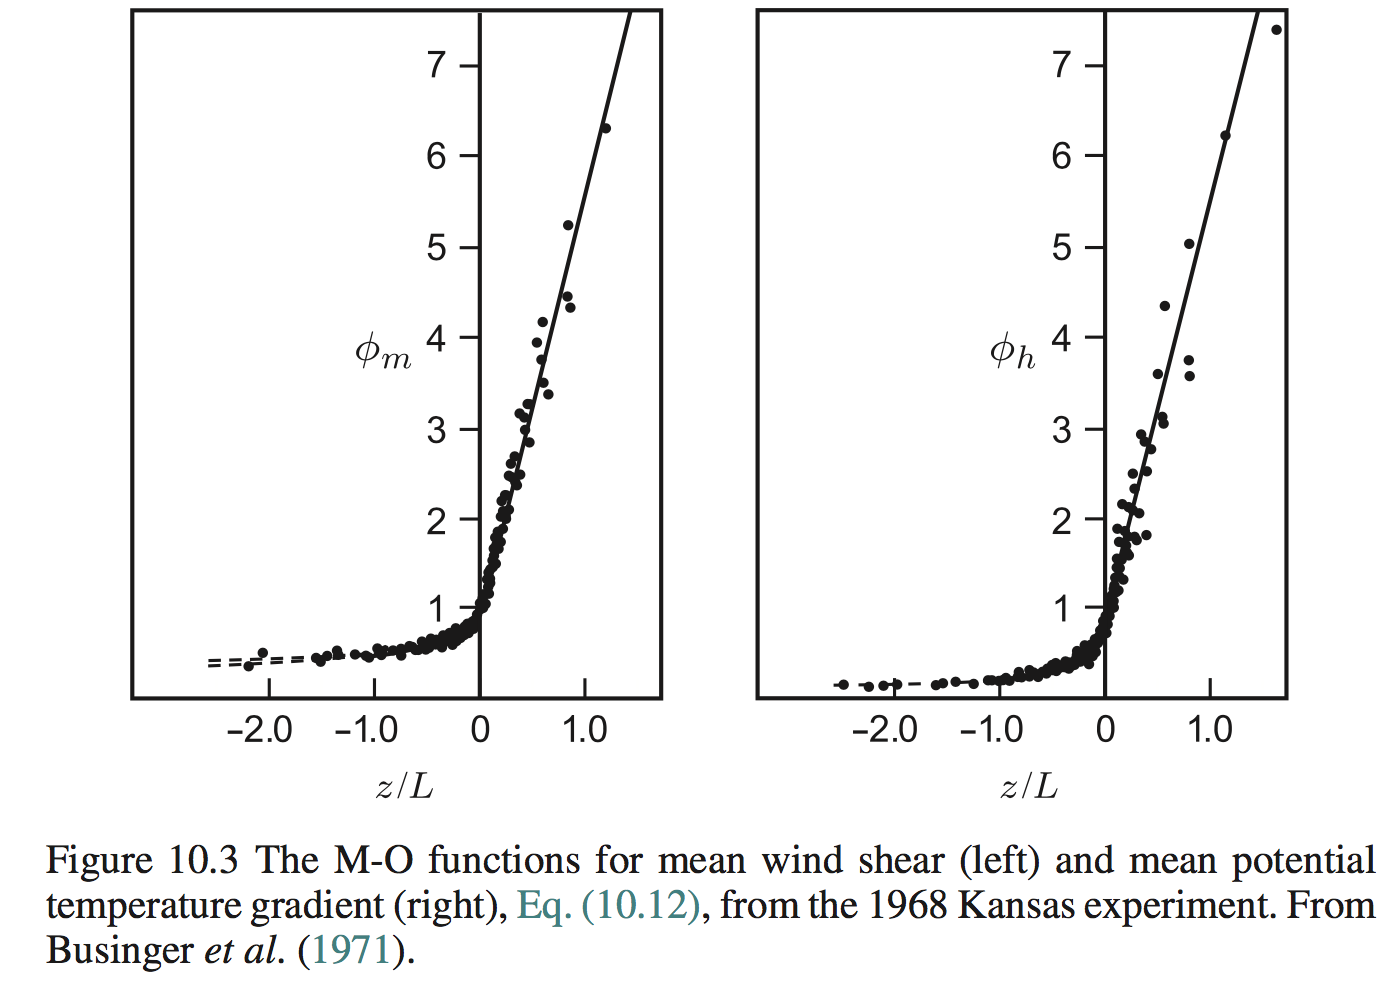
\includegraphics[width=0.8\textwidth]{mo1}	
		\end{figure}
		\tiny \centering From Wyngaard (2010)
	\end{itemize}
\end{frame}
%------------------------------------------------
\begin{frame}{Monin-Obukhov Similarity Theory}
	\begin{itemize}
		\item Although many forms exist, your professor prefers the functions proposed by Dyer (1974) because they are compact
		\begin{align*}
		\text{neutral} & \quad & \phi_m &= 1 & \quad  \phi_h &= 1\\
		\text{unstable} & \quad & \phi_m &= \left(1 - 16\zeta\right)^{-1/4} & \quad  \phi_h &= \left(1 - 16\zeta\right)^{-1/2}\\
		\text{stable} & \quad & \phi_m &= 1 + 5\zeta & \quad  \phi_h &= 1 + 5\zeta
		\end{align*}
	\item Thus, MOST allows us to determine turbulent fluxes from the mean gradients
	\end{itemize}
\end{frame}
%------------------------------------------------

\end{document}

